\documentclass[tikz,border=10pt]{standalone}
\usepackage{amsmath,amssymb}
\usetikzlibrary{arrows.meta,positioning}

\begin{document}
	
	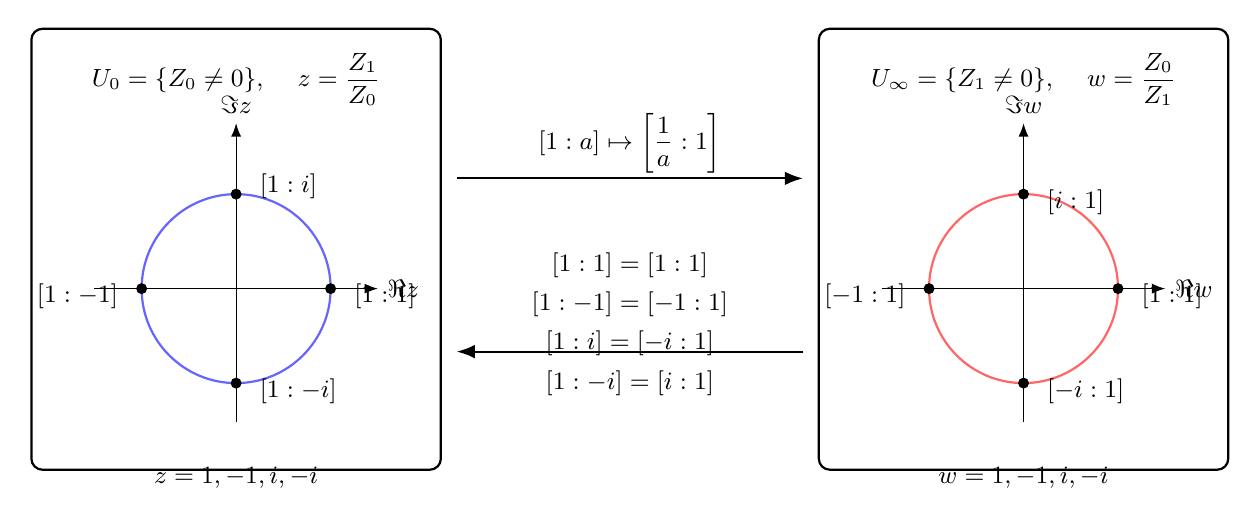
\begin{tikzpicture}[
		>=Latex,
		font=\small,
		point/.style={circle,fill=black,inner sep=1.4pt},
		box/.style={draw,rounded corners,thick,minimum width=5.2cm,minimum height=5.6cm},
		every node/.style={align=center}
		]
		
		% Left box: z-chart
		\node[box] (L) at (-5,0) {};
		\node[anchor=north] at ([yshift=-2mm]L.north)
		{\(U_0=\{Z_0\neq 0\}\), \quad \(z=\dfrac{Z_1}{Z_0}\)};
		
		\draw[->] (-6.8,-0.5) -- (-3.2,-0.5) node[right] {\(\Re z\)};
		\draw[->] (-5,-2.2) -- (-5,1.6) node[above] {\(\Im z\)};
		
		\draw[thick,blue!60] (-5,-0.5) circle (1.2);
		
		\node[point,label={[xshift=1mm,yshift=-1mm]right:\([1:1]\)}] at (-3.8,-0.5) {};
		\node[point,label={[xshift=-1mm,yshift=-1mm]left:\([1:-1]\)}] at (-6.2,-0.5) {};
		\node[point,label={[xshift=1mm,yshift=1mm]right:\([1:i]\)}] at (-5,0.7) {};
		\node[point,label={[xshift=1mm,yshift=-1mm]right:\([1:-i]\)}] at (-5,-1.7) {};
		
		\node at (-5,-2.9) {\(z=1,-1,i,-i\)};
		
		% Right box: w-chart
		\node[box] (R) at (5,0) {};
		\node[anchor=north] at ([yshift=-2mm]R.north)
		{\(U_\infty=\{Z_1\neq 0\}\), \quad \(w=\dfrac{Z_0}{Z_1}\)};
		
		\draw[->] (3.2,-0.5) -- (6.8,-0.5) node[right] {\(\Re w\)};
		\draw[->] (5,-2.2) -- (5,1.6) node[above] {\(\Im w\)};
		
		\draw[thick,red!60] (5,-0.5) circle (1.2);
		
		\node[point,label={[xshift=1mm,yshift=-1mm]right:\([1:1]\)}] at (6.2,-0.5) {};
		\node[point,label={[xshift=-1mm,yshift=-1mm]left:\([-1:1]\)}] at (3.8,-0.5) {};
		\node[point,label={[xshift=1mm,yshift=-1mm]right:\([i:1]\)}] at (5,0.7) {};
		\node[point,label={[xshift=1mm,yshift=-1mm]right:\([-i:1]\)}] at (5,-1.7) {};
		
		\node at (5,-2.9) {\(w=1,-1,i,-i\)};
		
		% Middle arrows
		\draw[->,thick] (-2.2,0.9) -- (2.2,0.9);
		\draw[->,thick] (2.2,-1.3) -- (-2.2,-1.3);
		
		\node at (0,1.35) {\([1:a]\mapsto \left[\dfrac1a:1\right]\)};
		\node at (0,-0.2) {\([1:1]=[1:1]\)};
		\node at (0,-0.7) {\([1:-1]=[-1:1]\)};
		\node at (0,-1.2) {\([1:i]=[-i:1]\)};
		\node at (0,-1.7) {\([1:-i]=[i:1]\)};
		
	\end{tikzpicture}
	
\end{document}